\chapter{How the First Cells Might Have Appeared}

\begin{kaichang}
At a riverbank or seashore, collect two things: a water-rounded pebble and a little creature crawling between stones, perhaps a woodlouse or small crab. Compare them in your palm. One stays motionless and would remain the same stone for a hundred years; the other crawls, eats, avoids you, and may later produce a brood.

\textbf{Translator safety note:} Make this comparison by observation or photographs, not by collecting or holding wild animals. Leave shore life undisturbed and follow local access and tide-safety guidance. See the \href{https://www.nps.gov/pore/planyourvisit/tidepooling.htm}{National Park Service's tidepool precautions}.

Now consider what they actually are. Chapter 7 said everything consists of atoms from the periodic table's hundred-odd elements. The stone is mostly silicon and oxygen; the creature mostly carbon, hydrogen, oxygen, and nitrogen. Both use the same box of building blocks. Why does one arrangement remain dead while another comes alive?

An even more exciting question follows. Four billion years ago, Earth had only rock, oceans, and air, not a single bacterium. Where did the first living thing come from? Guess an answer of your own. This chapter lays out both scientists' evidence and their gaps. You will encounter many instances of ``possibly'' and ``we do not yet know.'' That is not suspense for its own sake, but the honest state of the question.
\end{kaichang}

\section{Phenomena: Time Recorded in Rocks}

First inventory what is actually present and measurable.

First, Earth's age. Radioisotope dating from Chapter 8 gives the oldest meteorites and Moon rocks the same general message: the solar system and Earth formed about 4.54 billion years ago. This is not guesswork but agreement among several independent clocks, such as uranium decaying to lead.

Second, water arrived surprisingly early. Tiny zircon crystals from Western Australia's Jack Hills reach ages of 4.4 billion years. Their oxygen-isotope ratios suggest liquid water may already have existed near the surface when they formed. Oceans may therefore have appeared within a few hundred million years of Earth's birth.

Third, life appeared unusually quickly. The Pilbara region of Australia preserves roughly 3.5-billion-year-old stromatolites, layered rocks resembling cut cabbages, thought to record ancient microbial communities repeatedly growing and trapping sediment. Greenland has possible stromatolites about 3.7 billion years old and biologically suggestive carbon-isotope signals in 3.8-billion-year-old rocks, though these earlier claims remain disputed. Even accepting only the conservative 3.5-billion-year evidence, the conclusion is startling: only a few hundred million years, perhaps less, separate oceans from traces of life. On geological scales, it is almost as though life arrived soon after water gathered.

Fourth, the earliest records have permanently missing pages. Plate tectonics continually recycles, melts, and remakes Earth's surface, leaving almost none of its four-billion-year-old oceans and crust. The most direct evidence of when, where, and how life began was destroyed by Earth itself. That is the fundamental reason this chapter must keep saying ``possibly.''

A further important site appeared in 1977: deep-sea hydrothermal vents. Near the Galápagos, scientists in a submersible first saw black smokers along a seafloor rift, discharging scalding dark water loaded with mineral particles. Even more astonishing were dense communities of tube worms, clams, and shrimp. Their ecosystem depended on no sunlight, only bacteria consuming chemicals such as hydrogen sulfide and hydrogen. Life could evidently thrive without the Sun; reactions between rocks and water could support an entire city. This supplied a living model for the hypothesis of a seafloor origin.

\section{Particles: Gather the Parts First}

At molecular scale, make a construction list. Chapters 45--55 introduced life's main molecules: proteins are amino-acid chains in Chapter 48, membranes are largely lipids in Chapter 47, hereditary information is in nucleotide chains, and sugars supply fuel and materials in Chapter 46. The question becomes concrete: \textbf{could amino acids, lipids, and nucleotides arise spontaneously from an inorganic environment on a lifeless Earth?}

We now know at least three sources, each backed by evidence.

First, the sky. Early Earth lacked an ozone layer, so ultraviolet light reached the surface directly; volcanic eruptions, lightning, and impacts were also much more frequent. In such energetic conditions, simple gases could react into more complex small organic molecules. The evidence box soon tells the famous experimental story.

Second, the seafloor. Vents continually discharge hot water rich in hydrogen and mineral particles into cold seawater containing \chem{CO_2}. Porous mineral walls provide countless tiny reaction vessels, while mineral surfaces act as catalysts. Recall Chapter 30: catalysts do not change reaction direction, only provide easier routes. Scientists have detected simple organics at vents and synthesized fatty-acid-like molecules under simulated vent conditions.

Third, deliveries from space. The Murchison meteorite, which fell in Australia in 1969, contains more than 70 amino acids, most not among the 20 used by terrestrial life. That very difference indicates extraterrestrial chemical synthesis rather than contamination from Earth. Thousands to tens of thousands of tonnes of cosmic dust still reach Earth annually; early Earth would have received more.

All three sources support one conclusion: \textbf{the parts are not the problem}. Small organic molecules form in nonliving environments, a measurable fact rather than speculation. The real difficulty is the next step.

\begin{zhengju}
In 1952, University of Chicago graduate student Stanley Miller, supported by his adviser Harold Urey, built a glass apparatus. A heated water flask served as the ocean; a larger flask containing methane, \chem{CH_4}, ammonia, \chem{NH_3}, hydrogen, \chem{H_2}, and water vapor represented the primitive atmosphere. Two electrodes continuously sparked to imitate lightning. The sealed circulating system ran for a week.

A week later, the ocean was reddish brown. Analysis found glycine, alanine, and other amino acids: protein building blocks had appeared spontaneously from a mixture of inorganic gases. Publication in 1953 caused a sensation. The origin of life seemed overnight to become an experimentally accessible chemical question instead of a philosophical one.

But the interesting part was only beginning. Later research challenged Miller's atmospheric mixture. Growing evidence favored an early atmosphere dominated by \chem{CO_2} and \chem{N_2}, much less reducing than methane and ammonia. Electrical discharges in this milder atmosphere yielded far fewer amino acids. Critics said Miller had simulated an Earth that never existed.

The story continued. After Miller's death, his student Jeffrey Bada found original sample vials stored since the 1950s, from experiments never analyzed. In 2008, modern instruments revealed that a volcanic-eruption simulation with added \chem{H_2S} had produced 22 amino acids, more than originally reported. Even if the global atmosphere was unsuitable, \textbf{local environments} near volcanoes and vents could still have been efficient parts factories.

Remember three lessons: a good experiment may rest on assumptions later revised; revising those assumptions does not erase the experiment's demonstration that inorganic substances can become organic parts; and scientific honesty includes rechecking samples fifty years old.
\end{zhengju}

\section{Rules: Why Dilute Soup Is Not Yet Life}

Scatter the parts into an ocean, and you have only an immensely diluted organic soup. Three obstacles separate that soup from a cell, each requiring rules you have already learned.

\textbf{Obstacle one: concentration.} Molecules must collide to react, but oceans are enormous. Scattering parts into them is like adding a spoonful of sugar to West Lake: the parts hardly meet. How dilute is too dilute? Let us calculate.

\begin{qiaoliang}
Imagine a vesicle 1 micrometer across, about the size of a modern bacterium, with a volume around $5\times 10^{-16}$ liters. At a component concentration of 1 millimole per liter, $10^{-3}$ moles, which is not especially dilute, how many molecules does it hold?

Its amount is $5\times 10^{-16}\times 10^{-3}=5\times 10^{-19}$ moles. Multiplying by $6.02\times 10^{23}$ molecules per mole gives about $3\times 10^{5}$, or three hundred thousand molecules. That sounds substantial, but a self-copying chain might require hundreds of correctly ordered parts. In an unbounded ocean soup, actual concentrations might be thousands or tens of thousands of times lower. Without concentration mechanisms, the chance of assembling complex molecules through collisions becomes discouragingly small.
\end{qiaoliang}

Fortunately, early Earth had familiar ways to concentrate things. Sun-dried tidal pools concentrate solutes, like salt crystallizing from a dish of brine on a windowsill in Chapter 25. Freezing seawater forces impurities into residual brine in ice cracks, sharply raising concentrations; thaw frozen sugar water, and the first mouthful is extremely sweet. Micrometer-sized pores in vent minerals act like countless small pots, each simmering its own soup.

\textbf{Obstacle two: a boundary.} Chapter 45 named having an inside and outside as life's first feature. Without a boundary, useful newly made molecules immediately disperse into the sea. The good news is that boundaries can appear uninvited. Chapter 47 described phospholipids and simpler fatty acids as molecules with water-loving and water-avoiding ends. In water, they spontaneously form little bilayer-membrane spheres, or vesicles. This is a physical consequence of the hydrophobic effect in Chapters 22 and 23, requiring no life. Laboratory groups including Jack Szostak's have shown that fatty-acid vesicles form spontaneously, grow when fed more fatty acids, and split in two under shear from flowing water. A membrane house grows and divides without a single gene.

\begin{center}
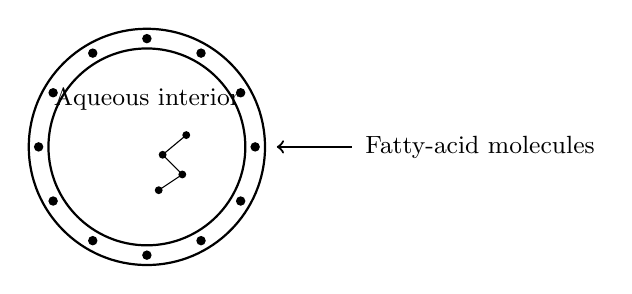
\begin{tikzpicture}
\draw[thick] (0,0) circle (1.5);
\draw[thick] (0,0) circle (1.25);
\foreach \a in {0,30,60,90,120,150,180,210,240,270,300,330} {
  \fill (\a:1.375) circle (0.06);
}
\draw (0.15,-0.55) -- (0.45,-0.35) -- (0.2,-0.1) -- (0.5,0.15);
\fill (0.15,-0.55) circle (0.05);
\fill (0.45,-0.35) circle (0.05);
\fill (0.2,-0.1) circle (0.05);
\fill (0.5,0.15) circle (0.05);
\node at (0,0.6) {\small Aqueous interior};
\draw[->,thick] (2.6,0) -- (1.65,0);
\node[right] at (2.65,0) {\small Fatty-acid molecules};
\end{tikzpicture}
\end{center}

Here, concentric circles represent a self-assembled fatty-acid bilayer, and the zigzag represents an enclosed nucleic-acid chain. This is purely a human representation: molecules are neither actual dots nor line segments.

\begin{shiyan}
\textbf{Materials:} two transparent cups, water, cooking oil, dishwashing liquid, and chopsticks.

\textbf{Procedure:} (1) Half-fill both cups with water, add 5 drops of cooking oil to each, stir each for 10 seconds with chopsticks, and leave to observe. (2) Add one drop of dishwashing liquid to the second cup, stir for another 10 seconds, and compare after standing.

\textbf{Observations:} without detergent, oil quickly gathers into round droplets of various sizes and floats up. Avoiding water, the molecules cluster to reduce contact area. With detergent, the oil breaks into more numerous, smaller, more stable droplets that resist merging. Detergent molecules have a water-loving end and an oil-loving end and surround each droplet like a molecular membrane. This illustrates amphiphilic molecules spontaneously creating boundaries: vesicles need no blueprint, only molecular properties and water's exclusion rules.

\textbf{Safety:} all materials are kitchen-grade and harmless; pour the finished liquid down the sink and rinse it away.

\textbf{Translator safety note:} Kitchen use does not make detergent harmless to swallow or splash in eyes. Use only the stated drop of hand-dishwashing liquid, never dishwasher detergent or another cleaner; do not taste the mixtures, and wash utensils and hands afterward. See \href{https://www.poison.org/articles/hand-dish-soap}{Poison Control's dish-soap precautions}.
\end{shiyan}

\textbf{Obstacle three: copying.} However beautiful a membrane house, without copying it is a one-off firework. Progress toward life requires a molecule that \textbf{carries information and uses it to copy itself}. Copying must also make mistakes, a counterintuitive but crucial point. Perfect copying yields repetition without change; imperfect copying produces variation, natural selection's raw material, explored in Volume III. Scribes make typos, repeated photocopies blur, and molecular copying likewise makes errors.

\section{Symbols: Meet DNA's Cousin First}

In your cells today, DNA stores information, proteins do most work, and RNA acts as messenger and tool in between, a system explored in Volume III. But look closely at this intermediary: RNA is unusual.

Like DNA, RNA is a long nucleotide chain. Each nucleotide contains phosphate, ribose, and one of four bases, A, U, G, and C. Chains obey strict pairing rules: A recognizes only U, and G only C, through the hydrogen-bond shape matching of Chapter 22, like complementary zipper teeth. Pairing lets one chain serve as a template for synthesis of a complementary chain. That is copying's chemical essence; Volume III's Chapter 66 examines DNA's version in detail.

Joining nucleotides removes one water molecule per added unit, like peptide-bond formation when amino acids become proteins in Chapter 48. Both are condensation reactions needing an energy push. This is obstacle three's tollbooth: template pairing is an information problem, while dehydration into chains is an energy problem. Both must be solved.

RNA's genuinely startling feature is that \textbf{it does not just carry information; it can work}. That is the next section's subject.

\section{The RNA World: Elegant but Unconfirmed}

Two independent discoveries shook biology in the 1980s. Studying Tetrahymena, Thomas Cech found an RNA that removed an internal segment and rejoined its ends without protein assistance. Sidney Altman showed that the catalytic worker in RNase P was its RNA component, with protein playing a supporting role. Catalytic RNAs were named \textbf{ribozymes}, and the two scientists received the 1989 Nobel Prize in Chemistry. An even greater surprise followed around 2000: high-resolution ribosome structures revealed that this protein-making machine's amino-acid-joining core is also RNA. Ultimately, every protein in your body is produced by RNA catalysis.

These discoveries inspired a bold idea: if RNA can both store information like DNA and catalyze reactions like enzymes, \emph{might an RNA world have preceded the division of labor between DNA and proteins}, with RNA handling both copying and catalysis in the first self-replicating systems? Walter Gilbert named the hypothesis in 1986. In this picture, stable DNA and versatile proteins are specialized departments that took over later; at the start, RNA played both roles.

Read this twice: \textbf{the RNA world is a hypothesis, not a historical recording already replayed}. Real evidence supports it: ribozymes exist, and ribosomal cores are RNA. It unifies many facts and is among the most influential pictures. But laboratories have recreated only \textbf{fragments}: some nucleotide ingredients under early-Earth-like conditions, a few short rounds of enzyme-free RNA copying, and growing, dividing vesicles. Nobody has joined these into a complete chain from inorganic matter to living cells. How were RNA parts made in bulk, how could enzyme-free copying become sufficiently long and accurate, and where did the first RNAs come from? The links remain unclosed.

\section{From Chemical to Darwinian Evolution}

Step back. Scientists broadly agree on what must come together between organic soup and first cells, but fiercely debate how and in what order. Consider four thresholds:

\begin{enumerate}[itemsep=2pt]
\item \textbf{An individual boundary:} a membrane vesicle separates a system from its environment so useful molecules accumulate as private resources instead of drifting away.
\item \textbf{Ways to obtain energy and materials from the environment:} primitive metabolism, perhaps reactions between vent hydrogen and \chem{CO_2} driving other reactions, a precursor of Chapter 50's energy-releasing/energy-consuming coupling.
\item \textbf{An information carrier that copies with errors:} for example, an RNA segment.
\item \textbf{Errors that affect copying success:} some vesicles have molecules that copy faster, or membranes that are stronger and less leaky.
\end{enumerate}

Once the fourth condition holds, natural selection starts \textbf{automatically}, without designer or commander. This is a statistical rule from Chapter 28: more successful replicators inevitably contribute a growing share of descendants, with differences amplified generation after generation. Chemical evolution, increasing molecular complexity under energy and probability rules, crosses into Darwinian evolution, where variations are selected and accumulate. The planet now has history: the next nearly four billion years unfold this logic, followed through evolution itself in Volume III.

Yet a major question remains unresolved, dividing researchers into camps: \textbf{which came first, metabolism or replication?} Replication-first approaches, broadly the RNA-world route, place copying molecules before vesicles and metabolism. Metabolism-first approaches begin with vent chemical energy driving simple reaction networks, primitive versions of Chapters 52 and 53's pathways, from which hereditary molecules later crystallized. Both have experimental support and unexplained gaps. Others suggest the two began intertwined rather than as alternatives. The honest answer is \textbf{we do not yet know}. That is science at work, not science failing.

\section{Limits: A Jigsaw, Not a Recording}

All this chapter's pictures---Miller's sky, vent pores, self-assembling vesicles, and an RNA world---are \textbf{possible routes consistent with existing evidence}, not claims that events definitely happened that way. There are three reasons.

First, Earth destroyed the direct evidence, so we cannot replay events. Second, every hypothesis has gaps: reliable enzyme-free copying for the RNA world, the bridge from reaction networks to heredity for vents, and perhaps even the identity of the protagonist, since simpler pre-RNA hereditary molecules have been proposed. Third, new evidence repeatedly revises the field, as Miller's atmospheric model warns us.

The model is useful because it shows life's origin \textbf{violates no physical or chemical law}, and its individual steps---self-assembly, catalysis, template copying, and natural selection---can be observed in laboratories. Its limitation is that it cannot be memorized as settled history. If a book announces that scientists have solved life's origin, remember this chapter, smile, and move on.

\begin{wuqu}
``Atoms randomly colliding into a cell would be like a tornado passing through a scrapyard and assembling a Boeing 747. It is probabilistically impossible, so a mysterious force must have intervened.''

The analogy fails twice. First, nobody proposes a cell arising in one collision. The picture involves countless \textbf{small steps}: vesicle self-assembly, gradual nucleotide formation, short-chain copying, then selection of replicators. Each is ordinary chemistry with a non-negligible probability, and products are retained by chemical rules and natural selection rather than dispersing after every collision. The tornado analogy substitutes a one-shot lottery for an accumulating process with memory and selection. Second, it implies ordered structures violate the second law. They do not: Earth is open, receiving energy continuously from the Sun and its interior. Local order is allowed if total entropy increases. Snowflakes, salt crystallization, and infant development are everyday examples from Chapter 28. The 747 analogy can warn against expecting everything at once, but misfires when used to dismiss an entire research field.
\end{wuqu}

\section{Back to the Pebble and the Creature}

We can answer the opening now. Pebble and creature use the same building blocks; every carbon and iron atom in the creature is as ancient as those in the stone. Chapter 16 explained that stars made the elements and Earth inherited them. The difference is \textbf{organization and history}. The creature contains countless membrane-bounded interiors, maintained day and night by energy flows from Chapters 50 and 53, plus information archives copied for nearly four billion years and bearing traces of copying errors. The stone has none: no inside--outside distinction, no energy flowing through, and nothing copying itself.

Life is therefore not a particular ingredient but a \textbf{way of operating}. How that operation first started among rocks and seawater remains open. This chapter offers the best available candidates and the most honest admission of what we do not yet know.

\section{Going Deeper: The Science an Open Question Supports}

You might not expect a field without a final answer to have produced practical fruit. Yet many drugs and vaccines use \textbf{liposomes} for delivery: artificial phospholipid vesicles enclose drugs and bring them safely to target cells. The core technology of mRNA vaccines packages mRNA in lipid nanoparticles. See the connection? A lipid vesicle enclosing nucleic acid is a technological version of our protocell sketch. Origin researchers make primitive vesicles, pharmacists delivery vesicles, using the same self-assembly principle.

Synthetic biology approaches from the other direction. Scientists have made artificial cells with genomes pared to a minimum, counting the least components a living system needs. Other teams evolve RNA populations through generations in test tubes, with real copying, variation, and selection. These are not replays of life's origin but maps of its possibility space.

The picture even changes the search for extraterrestrial life. If life can begin using chemical energy at vents, ancient Martian lake beds and the ocean beneath Europa's ice deserve investigation.

What did the first true cell look like, and how did it become today's bustling city with nucleus, mitochondria, and internal skeleton? Next chapter, we explore a modern cell. Living relics await: every ribosome still has an RNA core.

\begin{tiaozhan}
One mystery quietly omitted above is chirality. Chapter 42 described mirror-image molecules like left and right hands, while terrestrial life is extremely selective: proteins use almost only left-handed amino acids, and nucleic acids only right-handed sugars. Murchison's amino acids are nearly half left- and half right-handed, suggesting chemistry itself takes no side. Why and how did life choose? Perhaps chance: the first successful copying system used one hand and locked descendants into an inherited assembly line, like railway gauge that becomes expensive to change once laid. Others have found mechanisms amplifying small asymmetries, involving crystal surfaces or circularly polarized light in space, so the choice may not have been a coin toss. No final answer exists. Take this as a reminder: if even life's molecular handedness remains unexplained, origin research is far from finished.
\end{tiaozhan}

\section*{Practice}

\begin{sikaoti}
\item Draw a material-flow map from inorganic small molecules such as \chem{CO_2}, water, and \chem{N_2} to a membrane vesicle containing copying molecules. Label each arrow with its energy source, such as light, heat, or chemical energy, or its governing rule, such as hydrophobic effects or base pairing.
\item Replacing Miller's atmosphere with \chem{CO_2}, \chem{N_2}, and water vapor greatly lowers amino-acid yield. Use Chapters 27 and 29 to explain why changing reactants affects both how much can form and how fast it forms. What determines each?
\item Someone claims that drying a tidal pool concentrates dilute molecular soup, decreasing entropy and violating the second law. Refute this in three sentences using Chapter 28.
\item Szostak's fatty-acid vesicles grow and divide but are not yet alive. Which of this chapter's four thresholds are missing, and why can natural selection not begin without them?
\item How does calling the RNA world a scientific hypothesis differ from casually saying ``I have a hypothesis,'' meaning a guess? Use two examples from the evidence stories to identify the boundary.
\item Suppose vents and simple organic molecules are found beneath Europa's ice, but no copying molecules are detected. In this chapter's picture, how far through the four thresholds would that place the system?
\end{sikaoti}
